\documentclass[12pt, a4paper]{article}
\usepackage[polish]{babel}
\usepackage[utf8]{inputenc}
\usepackage[T1]{fontenc}
\frenchspacing
\usepackage{indentfirst}
\usepackage{amsfonts}
\usepackage{subcaption}
\usepackage{comment}
\usepackage{hyperref}
\usepackage{graphicx}
\usepackage[hang,flushmargin]{footmisc} 

\hypersetup{
    colorlinks  =   true,                   
    linkcolor   =   black,                  
    citecolor   =   black,                  
    urlcolor    =   blue                    
}
\urlstyle{same}

\title{Mobilne systemy informatyczne \\\normalsize\textbf{Projekt i implementacja systemu mobilnego}}
\author{Krzysztof Radosław Osada}
\date{\today}

\begin{document}
\maketitle

\tableofcontents
\newpage

\section{Wprowadzenie}
Niniejszy dokument jest omówieniem projektu i implementacji prostego \textbf{systemu mobilnego}. Praca jest zbudowana z czterech głównych sekcji: w~pierwszej z nich zawarty został wstęp do tematu, w drugiej -- informacje na temat projektu, w trzeciej -- dokumentacja ułatwiająca korzystanie z~systemu, natomiast w czwartej -- dane dotyczące implementacji.

\subsection{Podstawowe definicje}
W celu odpowiedniego zrozumienia przedstawianego problemu niezbędne wydaje się wypunktowanie kilku istotnych dlań pojęć:
\begin{itemize}
    \item \textbf{system mobilny} składający się zarówno z elementów stałych, jak i~ruchomych: użytkowników, serwerów oraz stacji bazowych;
    \item \textbf{użytkownicy}, mobilni, najczęściej przemieszczający się, korzystający z urządzeń bezprzewodowych i m.in. pod tym względem różnorodni (mający smartfony, palmtopy czy nawet radiowozy policyjne);
    \item \textbf{serwer}, komputer stacjonarny świadczący usługi na rzecz użytkowników znajdujących się w sieci;
    \item \textbf{stacja bazowa} zapewiająca utrzymanie łączności pomiędzy użytkownikiem a serwerem.
\end{itemize}

Wśród cech charakterystycznych systemów mobilnych wymienić można: brak wspólnej pamięci i globalnego zegara, komunikację ograniczoną do wymiany wiadomości czy asynchronizm wykonywanych operacji.

Połączenia w systemach mobilnych mogą być przewodowe bądź bezprzewodowe -- do tych ostatnich zalicza się: podczerwone, radiowe, ultradźwiękowe, mikrofalowe i laserowe.

Cennym źródłem informacji na temat systemów mobilnych są materiały dydaktyczne Wydziału Matematyki, Informatyki i Mechaniki Uniwersytetu Warszawskiego\footnote{\ M. Sobczak. Systemy mobilne - Studia Informatyczne. \url{http://wazniak.mimuw.edu.pl/images/1/11/Systemy_mobilne_wyklad_2.pdf}. Dostępny: 24.03.2018.}.

\subsection{Opis świata rzeczywistego}
Od zarania dziejów jedną z podstawowych życiowych potrzeb człowieka jest wzmacnianie jakości codziennej egzystencji. Nie bez przyczyny jedno z~polskich powiedzeń mówi, że potrzeba jest matką wynalazków; wiele odkryć w nauce i technice było wynikiem nie tylko ciekawości jednej osoby czy grupy ludzi, ale także jednoznacznym pragnieniem znalezienia sposobu na łatwiejsze wykonywanie jakiejś czynności. Nie inaczej było w informatyce.

Czytanie książek przez wieki było przywilejem -- aktywnością zarezerwowaną jedynie dla wąskiej grupy ludzi, którzy, będąc w większości ludźmi dobrze urodzonymi, mieli w życiu wystarczająco dużo szczęścia (i pieniędzy), aby zdobyć przynajmniej podstawowe wykształcenie i, co za tym idzie, posiąść umiejętność czytania. Przed ledwie stu laty z analfabetyzmem, czyli nieumiejętnością pisania i czytania oraz wykonywania podstawowych działań matematycznych, borykała się przeszło $33\%$ polskiego społeczeństwa\footnote{\ dzieje.pl. \textit{Historia Polski. Analfabetyzm w II Rzeczypospolitej}. \url{http://dzieje.pl/infografiki/analfabetyzm-w-ii-rzeczypospolitej}. Dostępny: 31.05.2018.}.

Spadek analfabetyzmu w Polsce i na świecie, czego konsekwencją było upowszechnienie umiejętności czytania -- spowodował wzrost popularności bibliotek. Według definicji instytucje te są ,,powołane od gromadzenia i udostępniania księgozbiorów''\footnote{\ PWN. Słownik języka polskiego. \url{https://sjp.pwn.pl/slowniki/biblioteka.html}. Dostępny: 31.05.2018.}; w praktyce dzięki takim miejscom możemy ,,wypróbować'' rozmaite książki, tzn. przejrzeć je albo nawet przeczytać bez konieczności posiadania ich na własność. Biblioteki mogą być przeznaczone dla ogółu ludzi zamieszkujących dane terytorium (np. Miejska Biblioteka Publiczna we Wrocławiu), pracowników i studentów wybranej uczelni (np. biblioteka Politechniki Wrocławskiej) czy wreszcie zawierać zbiory specjalne i~cenne pod względem dziedzictwa kulturowego (np. Biblioteka Ossolineum).

Podobnie jak w innych dziedzinach życia codziennego, nauki, biznesu i~czasu wolnego, tak i rynek biblioteczny został wzbogacony o rozmaite rozwiązania techniczne. Pierwsze systemy biblioteczne, których głównym celem jest możliwie jak najbardziej rozległa automatyzacja procesu wypożyczania książek i tworzenia księgozbiorów, pojawiły się już w latach 70. XX wieku\footnote{\ Wikipedia. \textit{Integrated library system}. \url{https://en.wikipedia.org/wiki/Integrated_library_system}. Dostępny: 31.05.2018.}. Obecnie nie są rzadkością usługi sieciowe umożliwiające przeglądanie zasobów bibliotecznych i wykonywanie określonych akcji, takich jak np. rezerwowanie i wypożyczanie książek czy tworzenie i blokowanie kont. Standardem stało się również oprogramowanie dedykowane dla całych sieci bibliotek; mamy wreszcie czytniki kodów kreskowych, QR code'ów i karty biblioteczne łudząco podobne do tych debetowych. Informatyka i nowoczesne technologie stały się nieodłączną częścią niemal wszystkich istniejących bibliotek\footnote{\ Niektóre filie biblioteki Politechniki Wrocławskiej do dnia dzisiejszego (31.05.2018) obsługują wypożyczenia książek bez użycia systemu informatycznego.}, aczkolwiek niektóre procesy, takie jak autentyfikacja użytkownika i wydawanie książek, pozostają -- z nie do końca jasnych przyczyn -- zinformatyzowane w~niewielkim stopniu i należą do obowiązków osób zatrudnianych przez biblioteki.

Wiodącą biblioteką we Wrocławiu jest wspomniana już \textbf{Miejska Biblioteka Publiczna}, mająca 38 filii\footnote{\ Miejska Biblioteka Publiczna we Wrocławiu.\\\url{http://www.biblioteka.wroc.pl/}. Dostępny: 31.05.2018.} zlokalizowanych na terenie całego miasta. Ważnymi instytucjami są także biblioteki uniwersyteckie, zlokalizowane przy Uniwersytecie Wrocławskim, Politechnice Wrocławskiej, Uniwersytecie Ekonomicznym, Uniwersytecie Przyrodniczym i innych szkołach wyższych. Każda z bibliotek posiada własną stronę internetową, za której pośrednictwem możliwe jest zarówno przeszukiwanie księgozbioru, jak i wypożyczanie książek; czynność tę należy jednak rozumieć jako \textit{wyrażenie chęci} wypożyczenia książki -- dopóki użytkownik nie pojawi się fizycznie w bibliotece i,~co bardziej istotne, nie potwierdzi swojej tożsamości, dopóty wybrana pozycja nie zostanie mu udostępniona. Ewentualna bierność, tzn. nieodebranie książki w terminie, może dodatkowo wiązać się z wystąpieniem czasowych bądź stałych blokad konta.

Wymienione strony internetowe bibliotek -- i kryjące się za nimi systemy informatyczne -- działają w gruncie rzeczy poprawnie: realizują bowiem swoje dwie wymienione wyżej podstawowe funkcje, dzięki którym użytkownik oszczędza czas, który dotąd musiał zużyć na znajdowanie interesującej go książki w katalogu i zgłaszanie jej wypożyczenia. Z drugiej jednak strony \textit{otoczenie}, w którym te procesy są wykonywane, wydaje się w niektórych przypadkach być zupełnie nieprzyjazne dla użytkownika i odstawać od aktualnych standardów. Możemy tu wymienić następujące problemy:\\

\noindent\textbf{Archaiczny wygląd}\\\vspace{-0.35cm}

Ważnym aspektem oceny produktu przez użytkownika są wywoływane u niego pozytywne (bądź negatywne) emocje. Mogłoby się wydawać, że subiektywne odczucia, które trudno jest w ogóle zmierzyć, nie mają większego wpływu na odbiór stron internetowych. Jest jednak przeciwnie -- dynamiczny rozwój nowoczesnych technologii WWW sprawił, że współcześnie kładzie się duży nacisk nie tylko na to, jakie funkcjonalności ma dostarczać dana aplikacja, ale też na to, w jaki sposób zaprezentuje ewentualne wyniki. Języki i biblioteki programowania pozwalają nam na zaprojektowanie aplikacji webowych o dowolnym wyglądzie, ale nie możemy zapomnieć o uwzględnieniu użyteczności, ergonomii i intuicyjności wdrażanych rozwiązań\footnote{\ Comarch. \textit{User Experience -- projektowanie pozytywnego doświadczenia}.\\\url{https://www.comarch.pl/erp/nowoczesne-zarzadzanie/numery-archiwalne/user-experience-projektowanie-pozytywnego-doswiadczenia/}. Dostępny: 31.05.2018.}. 

Niestety, ogólnie rozumiane \textit{doświadczenia} użytkownika są kwestią często pomijaną w funkcjonujących obecnie systemach bibliotecznych. \textbf{Politechnika Wrocławska} korzysta m.in. z systemu \textbf{Ex Libris} (Aleph) -- wprawdzie nie jest on dostępny bezpośrednio ze strony głównej biblioteki, ale jest na drugiej pozycji wyników wyszukiwania hasła \texttt{biblioteka pwr} w wyszukiwarce Google.

\begin{figure}[h]
    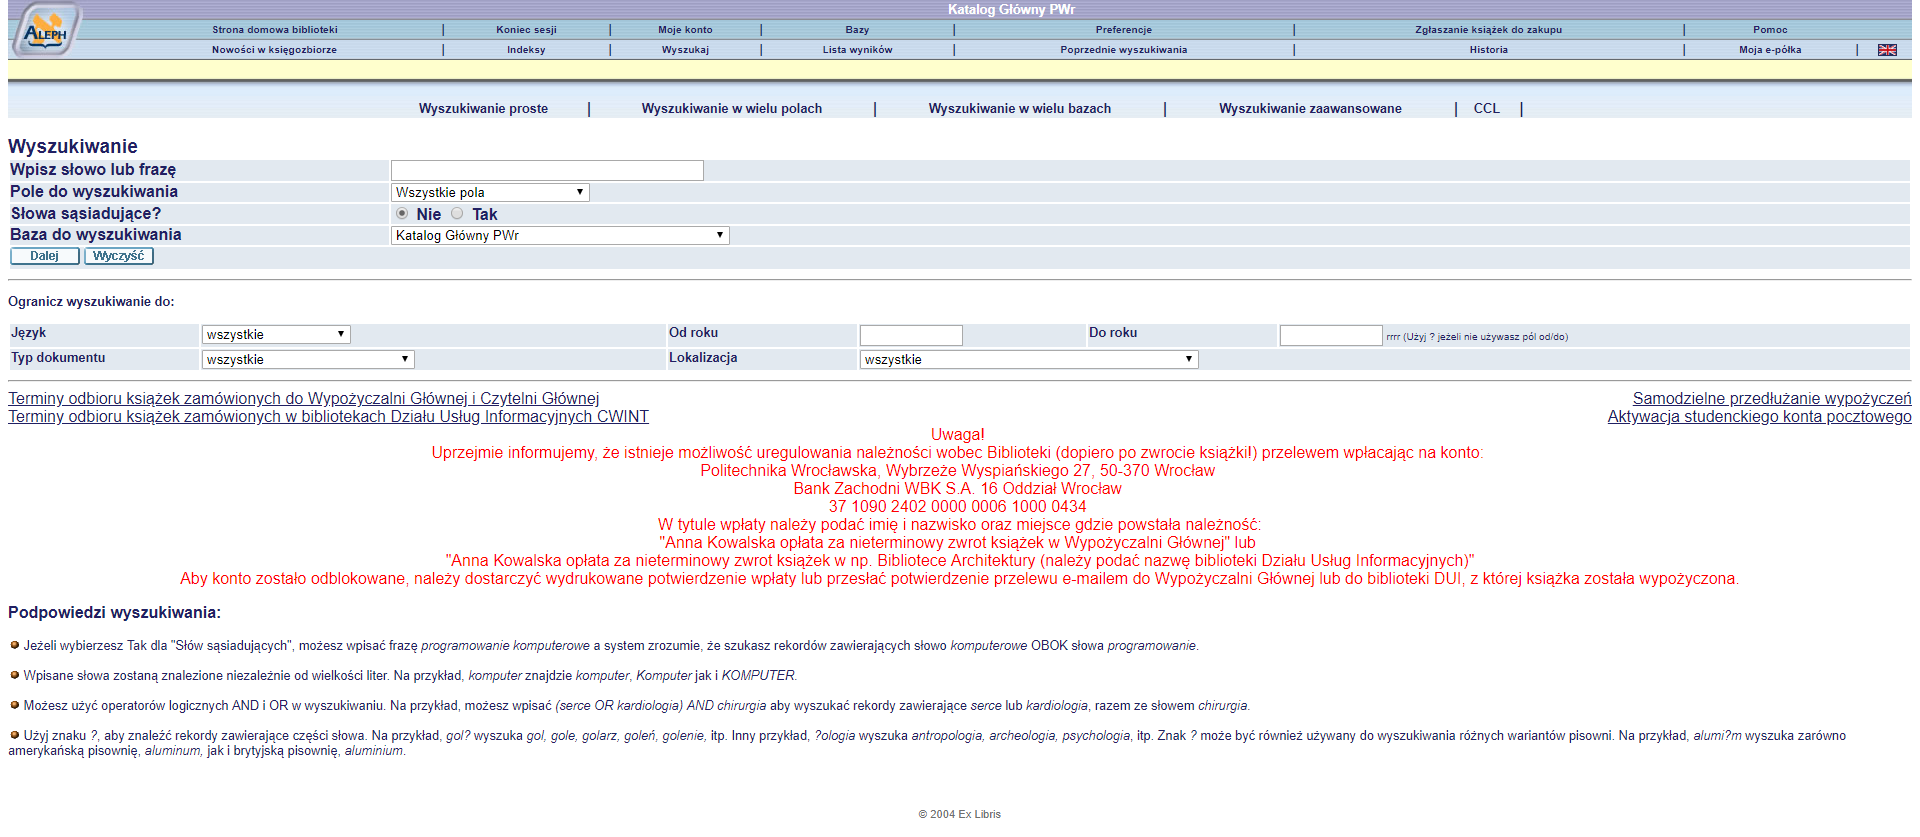
\includegraphics[width=\textwidth]{img/aleph.png}
    \caption{biblioteka PWr -- wygląd systemu Ex Libris (Aleph).}
\end{figure}

W tym przypadku trudno jest mówić o choćby częściowym dostosowaniu strony do oczekiwań potencjalnego użytkownika -- witryna sprawia wrażenie, jakby jej wygląd został przygotowany kilkanaście lat temu i od tamtej pory nie ulegl większym zmianom. Co gorsza, widoczna w górnej części rysunku nawigacja jest mało intuicyjna i nie ułatwia użytkownikowi znajdować interesujących go informacji.\\

\noindent\textbf{Brak responsywności}\\\vspace{-0.35cm}

Coraz trudniej wyobrazić sobie świat bez smartfonów -- zaawansowanych technologicznie telefonów komórkowych mających niemal nieograniczony dostęp do szybkiego Internetu oraz możliwości porównywalne z komputerami. Statystyki pokazują, że użytkownicy urządzeń mobilnych stanowią już ponad połowę osób przeglądających zasoby sieci WWW\footnote{\ Statista. \textit{Mobile share of website visits worldwide 2018}. \url{https://www.statista.com/statistics/241462/global-mobile-phone-website-traffic-share/}. Dostępny: 30.05.2018.}. Warto przy tym zwrócić uwagę na to, jak bardzo dynamicznie rozwinął się rynek smartfonów -- jeszcze dekadę temu udział posiadaczy komórek w statystykach użytkowników Internetu był znikomy.

W odpowiedzi na zmieniające się trendy w Internecie powstało pojęcie \textit{responsive web design} -- idea, zgodnie z którą należy projektować aplikacje webowe i strony internetowe w ten sposób, by dobrze wyświetlały się na ekranach o różnej szerokości (stąd i na smartfonach). Bazowy styl strony powinien być dostępny dla najmniejszego okna, natomiast definicje dla większych ekranów mogą pojawić się później -- taka kolejność sprawi, że słabsze urządzenia przetworzą tylko te reguły, które są niezbędne, natomiast lepsze telefony i komputery ,,dotrą'' do odpowiednich dlań dyrektyw.
 
Podobnie jak inne \textit{standardy} i \textit{zalecenia} funkcjonujące w sieci Web, projektowanie stron internetowych w duchu RWD nie jest bynajmniej formalnie narzuconym nakazem. Negatywnym skutkiem tej sytuacji jest utrudniony dostęp do wielu aplikacji webowych z poziomu urządzeń mobilnych. Dla przykładu strona internetowa \textbf{Miejskiej Biblioteki Publicznej we Wrocławiu} przy mniejszej szerokości ekranu prezentuje się szczególnie niekorzystnie:

\begin{figure}[h]
    \centering
    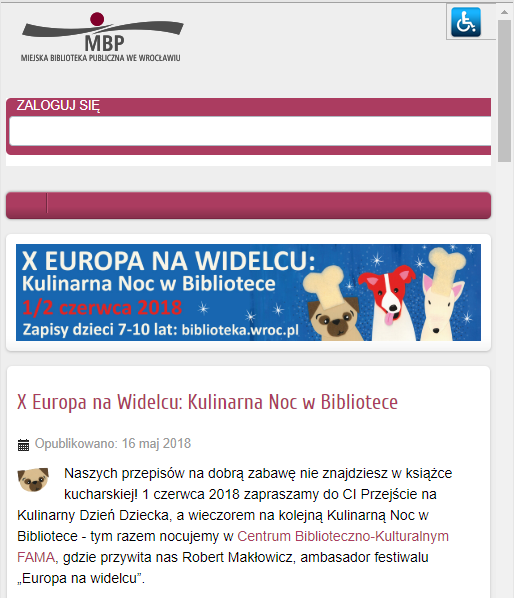
\includegraphics[width=0.5\textwidth]{img/mbp.png}
    \caption{MBP we Wrocławiu -- widok strony głównej.}
\end{figure}

Próżno tu szukać choćby nawigacji, w której znajdują się odnośniki do większości podstron portalu biblioteki; ponadto szerokość strony nie dostosowuje się do szerokości okna przeglądarki, a rozmiary czcionek są zbyt małe (co może sugerować, że nie ma w kodzie strony stosownej adnotacji o rozdzielczości ekranu). Wygląd witryny nie zachęca zatem do jej odwiedzin z~poziomu urządzenia innego niż komputer osobisty.

\subsection{Tematyka pracy}
Powyższa krótka, choć zarazem wyczerpująca analiza \textit{świata rzeczywistego} pozwala na wyciągnięcie podstawowych wniosków w tej kwestii. Jak widać, poważnym problemem środowiska bibliotecznego w mieście Wrocławiu od strony informatycznej jest jego zacofanie, które utrudnia bądź wręcz uniemożliwia zdalne korzystanie z dostępnych zasobów. To, że księgozbiory są dostępne za pośrednictwem Internetu, jest niezaprzeczalnym dobrem naszych czasów, jednak jakość tych usług pozostawia wiele do życzenia. Nie da się jednoznacznie ocenić, czy nieintuicyjny, archaiczny i nieprzyjazny dostęp do systemów bibliotecznych bezpośrednio wpływa na poziom czytelnictwa w~Polsce, który znacząco spadł w dobie Internetu i wynosi zaledwie 38\%\footnote{\ Biblioteka Narodowa. \textit{Stan czytelnictwa w Polsce w 2017 roku}. \url{http://instytutksiazki.pl/files/upload/files/Stan\%20czytelnictwa\%202017.pdf} Dostępny: 2.06.2018.}, ale z pewnością nie jest to czynnik sprzyjający.

Niniejszy dokument jest krótkim omówieniem implementacji prostego systemu bibliotecznego o nazwie \texttt{libsys} będącej zbitką dwóch wyrazów z języka angielskiego -- \textit{library} (pol. \textit{biblioteka}) oraz \textit{system}. Mimo że projekt ten nie jest bardzo innowacyjny pod względem przygotowanych funkcjonalności, ma jednak dużą, niepodważalną zaletę: \textbf{nowoczesny interfejs graficzny}, dostosowany do użytkowników różnej kategorii -- od posiadaczy smartfonów aż po właścicieli laptopów i komputerów stacjonarnych.

\section{Projekt}

Projekt był tworzony od marca do czerwca 2018 roku, natomiast jego dokumentacja powstawała na przełomie maja i czerwca tego samego roku. Osobą odpowiedzialną za rozwój \texttt{libsys} jest wyłącznie autor tej pracy. System został stworzony w celach edukacyjnych -- jego ukończenie nie jest planowane ze względu na inne cele i zobowiązania autora.

\subsection{Założenia}
Ogólną filozofię systemu można streścić w kilku hasłach:

\begin{itemize}
    \item \textbf{ładnie} -- wygląd aplikacji był jednym z najważniejszych aspektów rozważanych przy jej projektownaniu. Szablon \texttt{libsys} czerpie inspiracje z~rozwiązań przygotowanych przez profesjonalistów \href{https://www.w3schools.com/w3css/tryw3css_templates_interior_design.htm}{[1]}. Zastosowane zostały modne w dzisiejszym Internecie kontrastowe barwy, dobrane przy użyciu dedykowanych narzędzi.
    \item \textbf{mobilnie} -- jednym z głównych celów projektu jest udowodnienie, że systemy biblioteczne mogą być dostosowane do potrzeb zarówno użytkowników komputerów, jak i smartfonów. Interfejs graficzny \texttt{libsys} został przygotowany w oparciu o idee \textit{responsive web design}. Szablon strony przeznaczony dla urządzeń mobilnych nie jest jedynie dodatkiem, ale pełnoprawną wersją.
    \item \textbf{intuicyjnie} -- wyszukane rozwiązania i funkcjonalności ustąpiły miejsca prostocie i ergonomii. Autor projektu, będący notabene okazjonalnym miłośnikiem literatury, skupił swoją uwagę na zaprojektowanie takiego układu strony, który byłby łatwy w używaniu nawet przez mniej wprawnych odbiorców.
\end{itemize}

\textbf{Uwaga}. Projekt i jego implementacja stanowią jedynie \textit{zalążek} rozwiązania problemu -- \texttt{libsys} nie jest bowiem gotowym w pełni systemem bibliotecznym, tylko sugestią kierunku, w jakim powinny być rozwijane podobne projekty (w szczególności -- aplikacje webowe). Autor dokumentu jako wyłączny twórca systemu pragnie również podkreślić, że \texttt{libsys} nie jest wolny od błędów -- zarówno tych logicznych, jak i technicznych -- m.in. z powodu rozległości zagadnienia.

\subsection{Schematy i diagramy}
W tej części dokumentu prezentowane są rozmaite rysunki przedstawiające zbiory elementów i ilustrujące powiązania między nimi. Niektóre diagramy pochodzą z języka UML, wykorzystywanego m.in. do modelowania systemów. Literatura wymienia 9 podstawowych typów takich schematów\footnote{\ Booch G., Rumbaugh J., Jacobson I. \textit{UML. Przewodnik użytkownika}. Warszawa 2002.}; jednocześnie istnieją opinie, że trudno jest zdefiniować ,,uniwersalny zestaw'' diagramów adekwatnych do każdego rodzaju systemu\footnote{\ Pienkowski Rafal. \textit{Do developers still need UML?}. \url{https://dev.to/rafalpienkowski/do-developers-still-need-uml-ajh}. Dostępny: 3.06.2018.}. Z wyżej wymienionych powodów (a także ze względu na ograniczenia czasowe) wybrane zostały te diagramy, które wraz z rzeczowym opisem stanowią dobre źródło informacji na temat system.

\subsubsection{Diagram bazy danych}
Prawidłowe działanie systemu nie jest możliwe bez bazy danych, w której są gromadzone informacje na temat zarejestrowanych użytkowników, elementów księgozbioru czy wiadomości na blogu. W podstawowej wersji \texttt{libsys} niezbędna będzie baza danych zawierająca co najmniej \textbf{3 tabele} przedstawione na rysunku \ref{fig:dbdiagram}; wśród istotnych dla działania \texttt{libsys} pól rekordów są:

\begin{itemize}
    \item \texttt{users.id} -- unikalna dla każdego użytkownika liczba $n$ taka, że $n \in \mathbb{N} \land n > 0$, pozwalająca na jednoznaczne rozpoznanie osoby. Identyfikator jest używany we wszystkich tabelach. Pole to ma własność \texttt{AUTO\_INCREMENT} sprawiającą, że każda nowo dodana krotka posiada \texttt{id} większy o 1 od najwyższego dotychczas nadanego identyfikatora;
    \item \texttt{users.name} -- nazwa użytkownika, podobnie jak identyfikator, jest ograniczona do jednego rekordu w tabeli. Pole to jest używane zarówno przy autentyfikacji osoby (tzn. w procesie logowania), jak i prezentacji rozamitych danych (np. nick użytkowika, który wypożyczył daną książkę);
\end{itemize}

\begin{figure}[h]
    \centering
    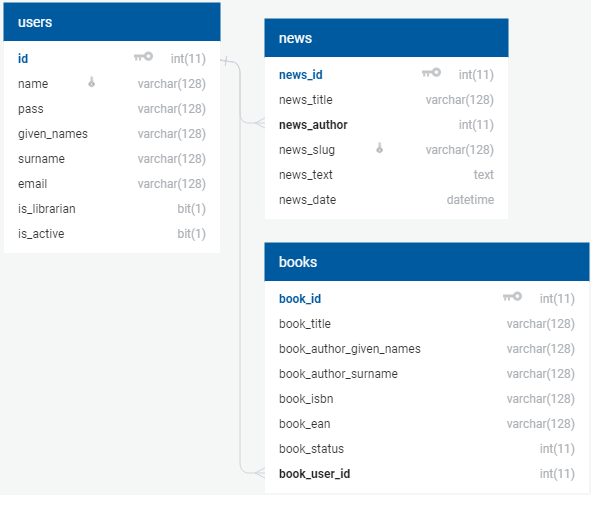
\includegraphics[width=0.9\textwidth]{img/diagram_db.png}
    \caption{struktura podstawowej bazy danych.}
    \label{fig:dbdiagram}
\end{figure}

\begin{itemize}
    \item \texttt{users.pass} -- hasło użytkownika. Należy pamiętać, że przechowywanie haseł w formie \textbf{tekstu jawnego} jest \textbf{całkowicie niedopuszczalne} -- podczas rejestracji albo zmiany hasła \texttt{libsys} szyfruje wprowadzony ciąg znaków i dopiero wtedy umieszcza go w bazie danych;
    \item \texttt{users.is\_librarian} -- pole typu logicznego (\texttt{true}/\texttt{false}) określające, czy użytkownik ma dostęp do przeznaczonej dla pracownika biblioteki i~wzbogaconej o dodatkowe funkcjonalności części systemu (zob. \ref{libsys_roles});
    \item \texttt{users.is\_active} -- pole typu logicznego (\texttt{true}/\texttt{false}) określające, czy konto użytkownika jest aktywne. Proces rejestracji w \texttt{libsys} zostaje uznany za zakończony jedynie wtedy, gdy użytkownik w odpowiednim czasie odbierze wysłany do niego e-mail i użyje odnośnika znajdującego się w treści wiadomości.
\end{itemize}

\subsubsection{Diagram klas}
\begin{figure}[h]
    \centering
    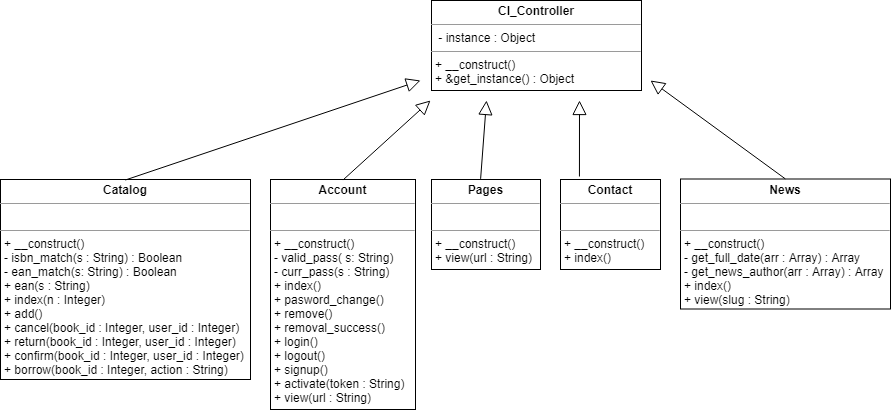
\includegraphics[width=\textwidth]{img/diagram_classes.png}
    \caption{diagram klas systemu.}
    \label{fig:classdiagram}
\end{figure}

W systemie zdefiniowanych jest 5 klas reprezentujących różne moduły -- są to:
\begin{itemize}
    \item \texttt{Account} -- moduł użytkownika;
    \item \texttt{Catalog} -- moduł biblioteczny;
    \item \texttt{Contact} -- podstrona formularza kontaktowego;
    \item \texttt{Pages} -- klasa ogólna dla zwykłych podstron;
    \item \texttt{News} -- mini-blog, czyli podstrona dla aktualności.
\end{itemize}
Klasy w \texttt{libsys} pełnią funkcję \textit{kontrolerów} -- przyjmują dane od użytkownika, zmieniają widok aplikacji i aktualizują modele. Więcej informacji dotyczących implementacji oraz funkcjonalności znajdują się kolejno w sekcjach \ref{libsys_technologies} oraz \ref{libsys_func}.

\subsubsection{Diagram przypadków użycia}
Przypadki użycia systemu są w większości skupione wokół modułów: bibliotecznego i użytkownika. Poniższy rysunek prezentuje podstawowe operacje wykonywane przez \textit{aktorów} (użytkowników) systemu:

\begin{figure}[h]
    \centering
    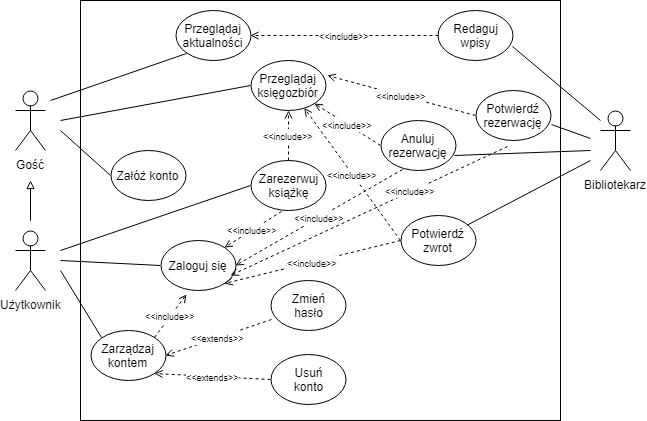
\includegraphics[width=\textwidth]{img/diagram_use_cases.png}
    \caption{diagram możliwych przypadków użycia \texttt{libsys}.}
    \label{fig:ucdiagram}
\end{figure}

Użytkownicy \texttt{libsys} przyjmują określone role różniące się zakresem uprawnień i ewentualnymi ograniczeniami dostępu do funkcjonalności. Sekcja \ref{libsys_roles} tej pracy przybliża typy użytkowników.

\subsubsection{Diagram stanów}
Jednym z najważniejszych i zarazem najbardziej podstawowych obiektów w systemie bibliotecznym jest książka -- wg definicji ,,złożone i oprawione arkusze papieru, zadrukowane tekstem literackim, naukowym lub użytkowym''\footnote{\ PWN. Słownik języka polskiego. \url{http://sjp.pwn.pl/szukaj/ksi\%C4\%85\%C5\%BCka}. Dostępny: 7.06.2018.}. Książka -- w zależności od tego, czy jest wypożyczona, czy też nie -- może znajdować się w różnym \textbf{stanie} (zob. sekcję \ref{libsys_book_status}). Pojęcie to dobrze obrazuje diagram \ref{fig:stdiagram}.

\begin{figure}[h]
    \centering
    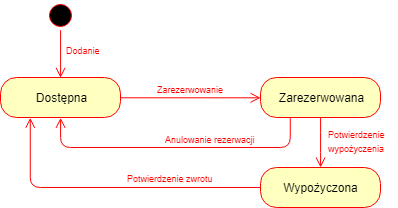
\includegraphics[width=\textwidth]{img/diagram_states.png}
    \caption{diagram możliwych stanów książki.}
    \label{fig:stdiagram}
\end{figure}

\subsection{Lista funkcjonalności}
\label{libsys_func}
Projekt \texttt{libsys} to luźna interpetacja systemu bibliotecznego -- jego istotną częścią jest zatem moduł do wypożyczania książek i przeglądania księgozbioru. Przygotowane przez autora rozwiązania można podzielić według kilku wymienionych poniżej kategorii.

\subsubsection{Konta}
Wypożyczenie książki jest -- jak by nie patrzeć -- zobowiązaniem polegającym na wejściu w tymczasowe posiadanie ruchomości należącej do innego podmiotu (osoby) i zwrócenie tej rzeczy w stanie niezmienionym. Ponieważ czynność ta wiąże się niejednokrotnie z poniesieniem ewentualnych kosztów finansowych, powinna być odpowiednio chroniona. Konta w \texttt{libsys} są zatem potrzebne do jednoznacznej \textbf{identyfikacji} użytkowników i przydzielenia im odpowiednich \textbf{uprawnień}. Na moduł użytkownika składają się:
\begin{itemize}
    \item rejestracja kont spełniających odpowiednie kryteria (silne hasło, poprawny adres e-mail itd.), aktywowanych przy użyciu linków o krótkiej ważności wysyłanych na podany adres elektroniczny (za pośrednictwem serwera \textbf{Gmail});
    \item autentyfikacja użytkownika poprzez sprawdzanie zgodności nazwy użytkownika i \textbf{zaszyfrowanego} hasła z informacjami przechowywanymi w~bazie danych;
    \item ograniczenie dostępu (ew. ukrycie części funkcjonalności) dla gościa (użytkownika niezalogowanego) na większości podstron;
    \item dodatkowe operacje: zmiany hasła i usunięcia konta.
\end{itemize}

\subsubsection{Typy użytkowników}
\label{libsys_roles}
W systemie bibliotecznym ważne jest rozgraniczenie kilku grup potencjalnych użytkowników; mają oni bowiem różne kompetencje, z których powinien wynikać odmienny zakres dostępnych funkcjonalności. W \texttt{libsys} zdefiniowane są trzy role:

\begin{itemize}
    \label{libsys_roles}
    \item \textbf{gość} -- dowolna osoba korzystająca z \texttt{libsys}, której ustalenie tożsamości nie jest możliwe. Użytkownik niezalogowany (niezarejestrowany) nie ma prawa do wykonywania żadnych operacji na księgozbiorze -- widzi jedynie jego zawartość;
    \item \textbf{użytkownik} -- dowolna osoba korzystająca z \texttt{libsys}, której tożsamość jest znana. Użytkownik może rezerwować książki i zmieniać podstawowe dane dotyczące swojego konta;
    \item \textbf{bibliotekarz} -- użytkownik posiadający specjalne uprawnienia. Stanowi on rolę kontrolną w systemie: potwierdza wypożyczenia i zwroty dokonane przez użytkownika, ale sam jest jednocześnie pozbawiony takich uprawnień. W implementacji wykrywany przy pomocy flagi \texttt{is\_lib-} \texttt{rarian};
\end{itemize}

\subsubsection{Biblioteka}
\label{libsys_book_status}
sModuł biblioteczny jest najważniejszą częścią systemu, jego \textit{clou} -- umożliwia wykonywanie rozmaitych operacji na księgozbiorze. Zdefiniowane zostały ponisze zadania:

\begin{itemize}
    \item \textbf{wyszukiwanie} książki z listy na podstawie jednej z jej cech:
    \begin{itemize}
        \item \textbf{tytułu lub jego fragmentu} -- wpisana przez użytkownika fraza (zob. rys. ) jest porównywana ze wszystkimi pozycjami dostępnymi w księgozbiorze. Wynikiem wyszukiwania powinny być wszystkie książki, których tytuł zawiera całą wpisaną frazę,
        \item \textbf{kodu EAN-13 (ISBN)} -- wysłane przez użytkownika zdjęcie zostaje poddane analizie pod względem zawartości. Jeśli na fotografii znajduje się kod w formacie EAN (ang. \textit{European Article Number}), to jego wartość jest wyszukiwana w księgozbiorze, analogicznie do tytułów w powyższym zdaniu;
    \end{itemize}
    \item \textbf{rezerwowanie} książki -- proces poprzedzający faktyczne wypożyczenie, polegający na zgłoszeniu zamiaru wypożyczenia danej pozycji. Podobna operacja jest w MBP we Wrocławiu znana jako \textit{zamówienie} książki;
    \item \textbf{wypożyczenie} książki -- operacja wykonywana przez bibliotekarza, ograniczająca się do potwierdzenia wypożyczenia danej książki. Odpowiednik tej czynności w świecie rzeczywistym to przekazanie czytelnikowi wypożyczonej książki do ręki;
    \item \textbf{anulowanie rezerwacji} książki -- zdarzenie przeciwne do wypożyczenia, także związane z rolą bibliotekarza. Może mieć ono miejsce na przykład wtedy, gdy użytkownik nie zrealizuje swojej rezerwacji w odpowiednim czasie;
    \item \textbf{potwierdzenie zwrotu} książki -- czynność realizowana przez bibliotekarza po oddaniu książki przez czytelnika. Dokonanie potwierdzenia zwrotu powoduje że książka ponownie widnieje w systemie jako dostępna i może ją wypożyczyć kolejna osoba. 
\end{itemize}

Z każdą książką w \texttt{libsys} wiąże się odpowiedni status:

\begin{itemize}
    \item \textbf{dostępna} -- żaden z użytkowników nie wypożycza danej pozycji;
    \item \textbf{zarezerwowana} -- jeden z użytkowników zgłosił zamiar wypożyczenia pozycji i ma na nią wyłączność (w skończonym czasie);
    \item \textbf{wypożyczona} -- książka nie będzie dostępna do momentu zwrócenia jej przez czytelnika.
\end{itemize}

\subsubsection{Dodatki}
Projekt zakłada, że \texttt{libsys} będzie zawierał także inne funkcjonalności, niezwiązane bezpośrednio z głównym zadaniami systemu. Proponowanymi przez autora rozwiązaniami są:

\begin{itemize}
    \item \textbf{interaktywna mapa} prezentująca w podstawowej wersji lokalizacje bibliotek zaprezentowane w graficznej formie (np. znaczników);
    \item \textbf{aktualności} -- niewielki blog pozwalający na dodawanie wiadomości. Wpisy prezentowane są we fragmentach na liście w odwróconym porządku chronologicznym. Istnieje także możliwość przeczytania pełnej treści wpisu (w osobnym widoku);
    \item \textbf{formularz kontaktowy} -- komponent służący do kontaktu z administratorem (autorem) systemu, dostępny zarówno dla gości, jak i dla zalogowanych użytkowników.
\end{itemize}

\section{Implementacja}
\subsection{Wykorzystywane technologie}
\label{libsys_technologies}
Prezentowana wersja \texttt{libsys} została zaimplementowana w formie aplikacji webowej pracującej na serwerze i komunikującej się z klientem za pośrednictwem przeglądarki internetowej. Swoje wykorzystanie w projekcie znalazły rozmaite technologie WWW, wśród których wymienić można między innymi:

\begin{itemize}
    \item \textbf{XAMPP 7.0.25} -- darmowy, wieloplaformowy pakiet typu \textit{open source} będący darmowym serwerem WWW do obsługi dynamicznych stron internetowych. Zestaw zapewnia bazę danych i interpetację plików PHP, z których w większości składa się \texttt{libsys};
    \item \textbf{CodeIgniter 3.1.8} -- prosty framework do budowy dynamicznych stron internetowych z PHP. CI może się szczycić czytelną składnią, przystępną dokumentacją i dużą społecznością użytkowników; 
    \item \textbf{HTML 5} z \textbf{CSS 3} -- języki stanowiące podstawę każdej nowoczesnej strony internetowej, używane do definiowania struktury blokowej dokumentów i nadawania im stylów;
    \item \textbf{jQuery 3.3.1} -- biblioteka ułatwiająca korzystanie z języka \textbf{JavaScript} i pisanie skryptów na stronach WWW, przydatna przede wszystkim przy tworzeniu zapytań AJAX i wyszukiwaniu elementów w dokumentach HTML;
    \item \textbf{Font Awesome 5.0.13} -- oparty o CSS i LESS zestaw ikon oraz logotypów będacy (według autorów) najpopularniejszym tego typu narzędziem na świecie\footnote{\ Font Awesome. \url{https://fontawesome.com}. Dostępny: 6.06.2018.};
    \item \textbf{QuaggaJS} -- zaawansowany czytnik kodów kreskowych napisany w języku JavaScript. Biblioteka mieści się w jednym pliku, nie wymaga dostępu do Internetu i rozpoznaje m.in. kody EAN-13 i ISBN, standardów powszechnie wykorzystywanych na rynku wydawniczym.
\end{itemize}

\newpage
\subsection{Interfejs użytkownika}

Szablon systemu \texttt{libsys} jest zbudowany z plików PHP, JS i CSS. Najistotniejsze części strony, wśród których można wymienić: nagłówek z panelem nawigacji, część główna oraz stopka, są zdefiniowane w osobnych plikach zwanych \textit{widokami}. Każda z podstron systemu stanowi niejako osobną \textit{klasę} i ma zdefiniowane unikalne dla siebie style i układy treści.

\textbf{Strona główna} aplikacji zawiera jedynie wiadomość powitalną, która łatwo może być rozszerzona o dodatkową treść. Istnieje również możliwość przekierowania na podstronę \textbf{aktualności}:

\begin{figure}[h]
    \centering
    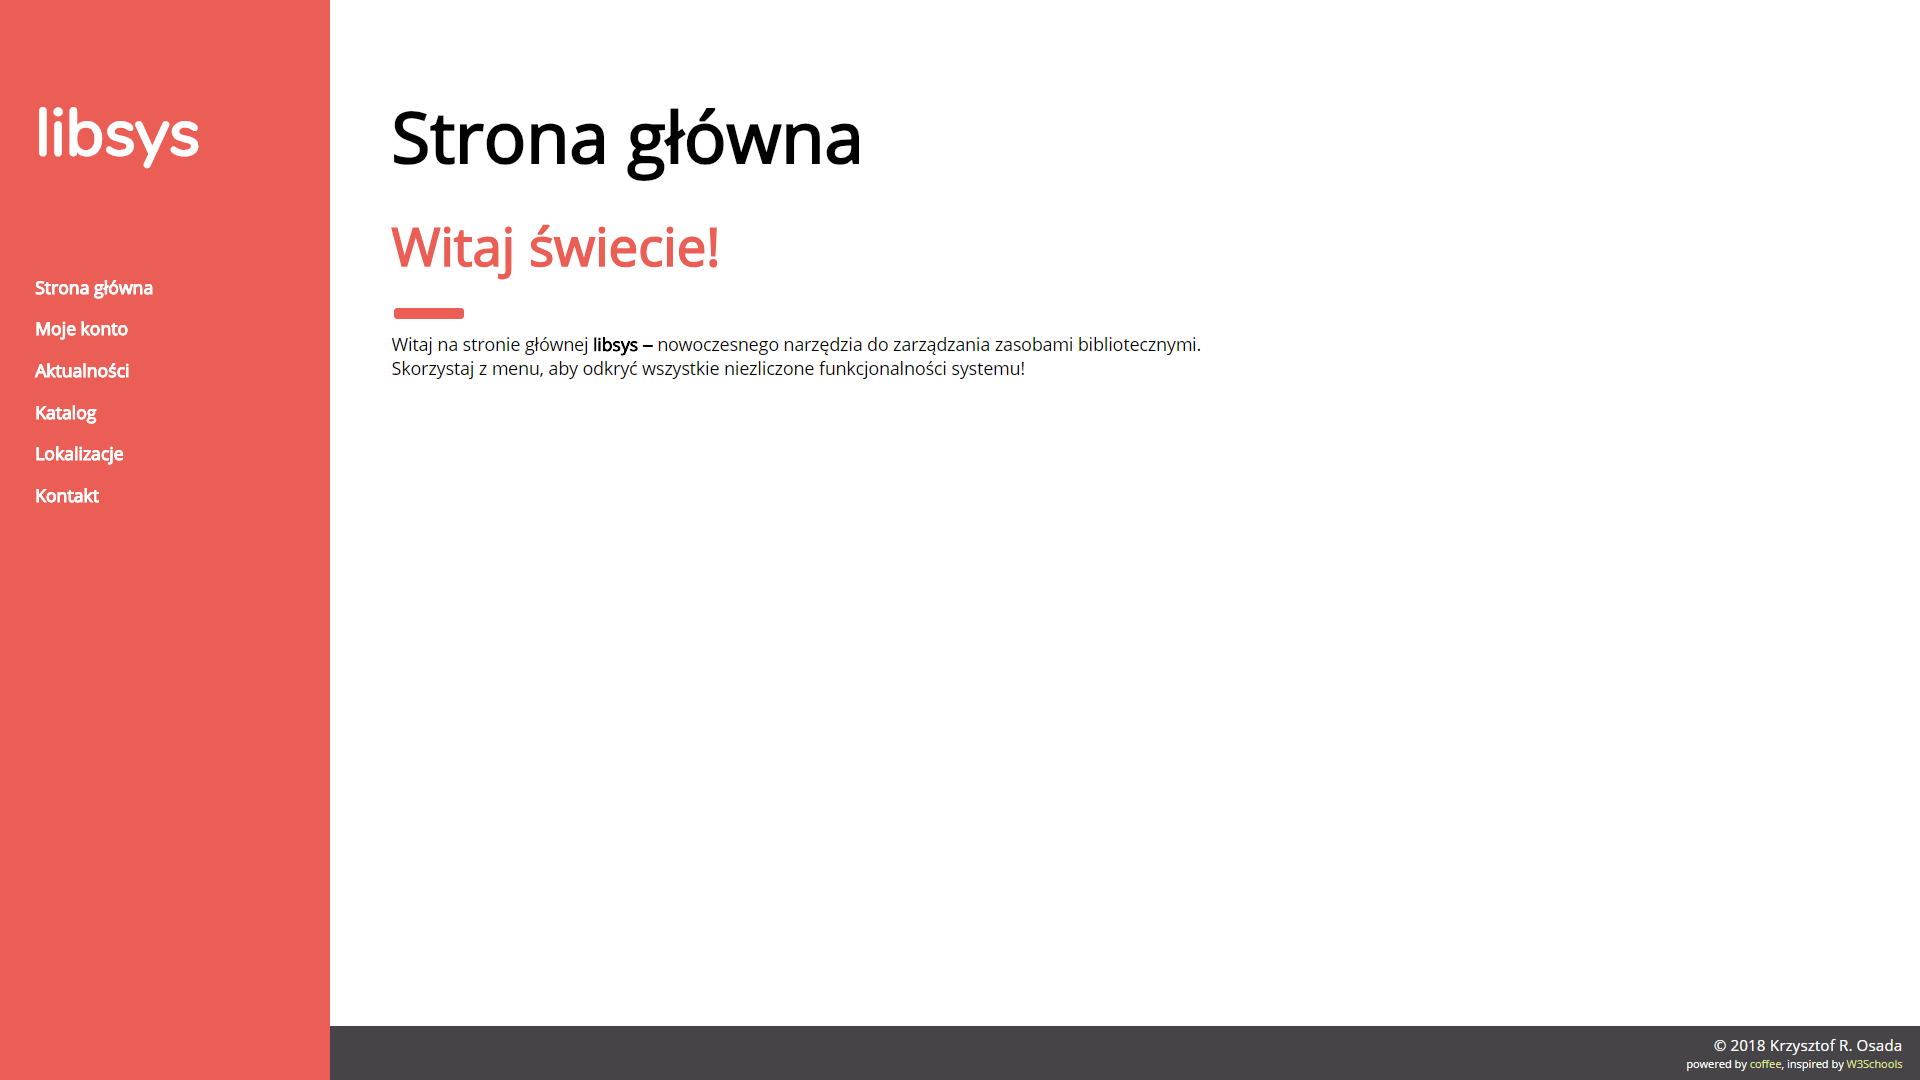
\includegraphics[width=\textwidth]{img/libsys_home.png}
    \caption{\texttt{libsys} -- strona główna.}
\end{figure}

\begin{figure}[h]
    \centering
    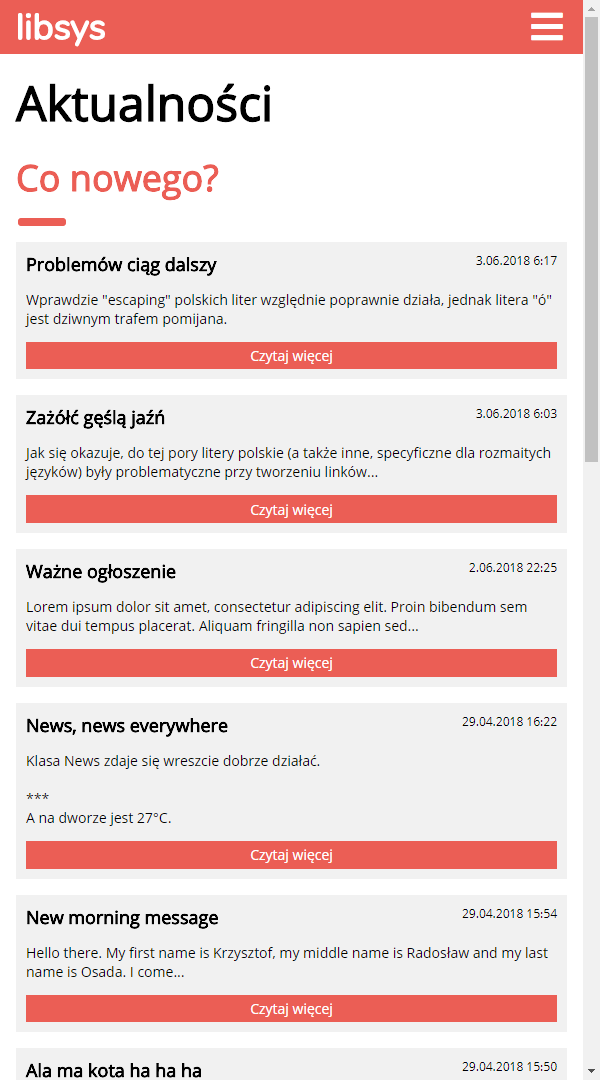
\includegraphics[width=0.4\textwidth]{img/libsys_news.png}
    \caption{\texttt{libsys} -- aktualności.}
\end{figure}

Jest ona swego rodzaju mini-blogiem, na której pojawiają się wpisy wyświetlane w kolejności od najnowszego do najstarszego. Naciśnięcie przycisku \texttt{Czytaj więcej} skutkuje przeładowaniem strony i wyświetleniem pełnej treści wybranej wiadomości. Na samym końcu listy wpisów znajduje się dodatkowy odnośnik prowadzący do strony dodawania newsów, pokazywany jedynie osobom do tego uprawnionym.

Dostęp do części funkcjonalności \texttt{libsys} jest dostępny jedynie po zalogowaniu. Próba nieuprawnionego wejścia skutkuje przekierowaniem na stronę \textbf{logowania}, gdzie użytkownik systemu wprowadza swoje dane: nazwę (login) oraz hasło. Poniżej formularza znajduje się link do podstrony rejestracji.

Pojawienie się ewentualnych błędów przy wprowadzaniu danych -- zarówno w formularzu logowania, jak i w innych miejscach -- powoduje, że system zwraca odpowiednie \textbf{komunikaty}. Wiadomości te prezentowane są w postaci niewielkich bloków tekstu w kontrastowym kolorze:

\begin{figure}[h]
    \centering
    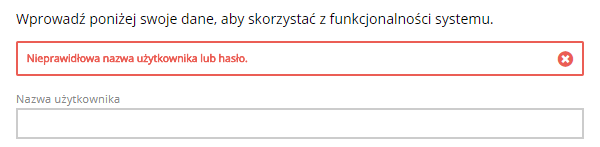
\includegraphics[width=\textwidth]{img/libsys_account_4.png}
    \caption{\texttt{libsys} -- komunikat o błędzie.}
\end{figure}

Jeżeli autentyfikacja jest zakończona się powodzeniem, następuje przejście do \textit{pulpitem} użytkownika -- podstrony, na której może on wykonać podstawowe operacje dotyczące swojego konta. 

\begin{figure}[h]
\centering
\begin{subfigure}{.4\textwidth}
    \centering
    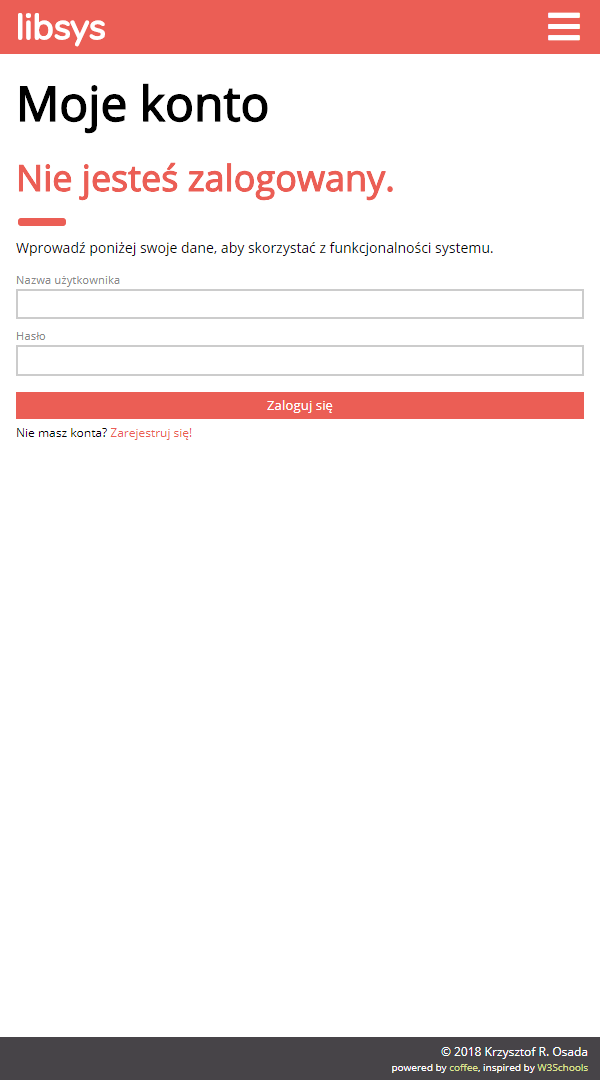
\includegraphics[width=.75\linewidth]{img/libsys_account_1.png}
\end{subfigure}\quad
\begin{subfigure}{.4\textwidth}
    \centering
    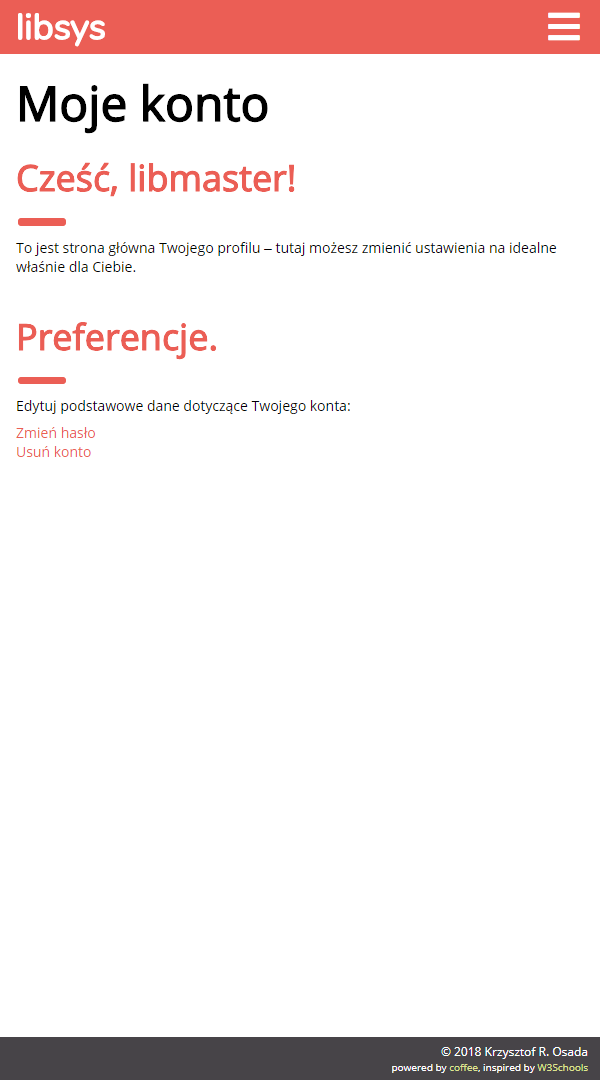
\includegraphics[width=.75\linewidth]{img/libsys_account_2.png}
\end{subfigure}
\caption{\texttt{libsys} - strona logowania / pulpit użytkownika.}
\end{figure}

Wybór opcji \textbf{zmiany hasła} skutkuje załadowaniem nowej strony, na której widnieje formularz z odpowiednimi polami. Jego wypełnianie to operacja łatwa i przyjemna -- wszystkie pola są opatrzone właściwym opisem, przycisk zapisu wyróżnia się kontrastowym kolorem, a~ewentualne błędy system przedstawia w postaci ostrzeżeń. Drugą dostępną w panelu użytkownika opcją jest usunięcie konta, które jest, rzecz jasna, całkowicie odradzane. Zamknięcie konta to operacja nieodwracalna -- wiąże się z utratą dostępu do części udogodnień systemu.

\textbf{Nawigacja} strony pomaga zorientować się w fukcjonalnościach \texttt{libsys}; jest niewielka, czytelna i -- co najważńiejsze -- zrozumiała. Menu w wersji systemu na urządzenia mobilne jest widoczne jedynie na żądanie, otwierane przy użyciu przycisku ukazanego w prawym górnym rogu rysunku (tzw. \textit{bars} albo \textit{hamburger}). Zabieg ten przekłada się na oszczędność miejsca na ekranie, która jest mocno ograniczona szczególnie w przypadku małych telefonów komórowych.

\begin{figure}[h]
    \centering
    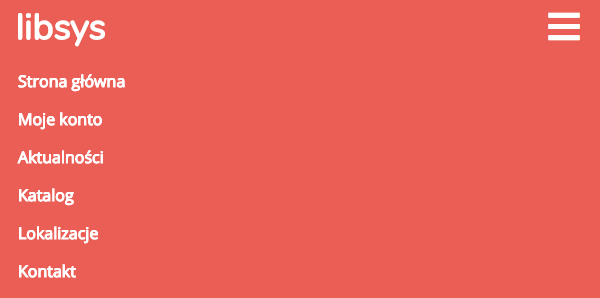
\includegraphics[width=.4\textwidth]{img/libsys_menu.png}
    \caption{\texttt{libsys} -- nawigacja.}
\end{figure}

Analogicznie wygląda formularz \textbf{kontaktowy} (rys. \ref{fig:libsys_contact}), względem pozostałych wzbogacony o duże pole tekstowe i umożliwiający wysyłanie zapytań związanych m.in. z działaniem systemu:

\begin{figure}[h]
\centering
\begin{subfigure}{.4\textwidth}
    \centering
    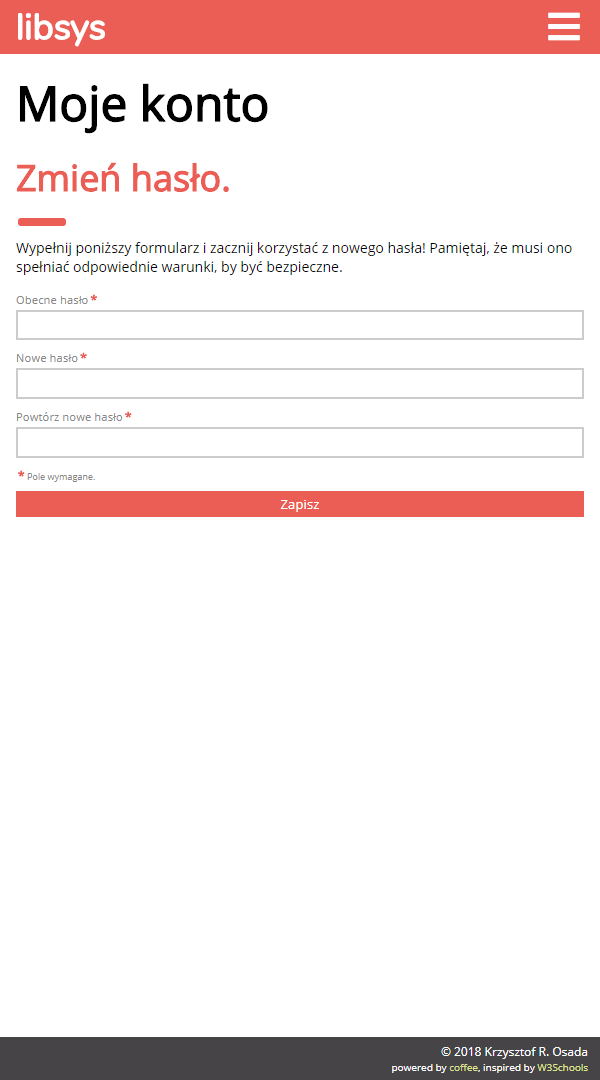
\includegraphics[width=.75\linewidth]{img/libsys_account_3.png}
\end{subfigure}\quad
\begin{subfigure}{.4\textwidth}
    \centering
    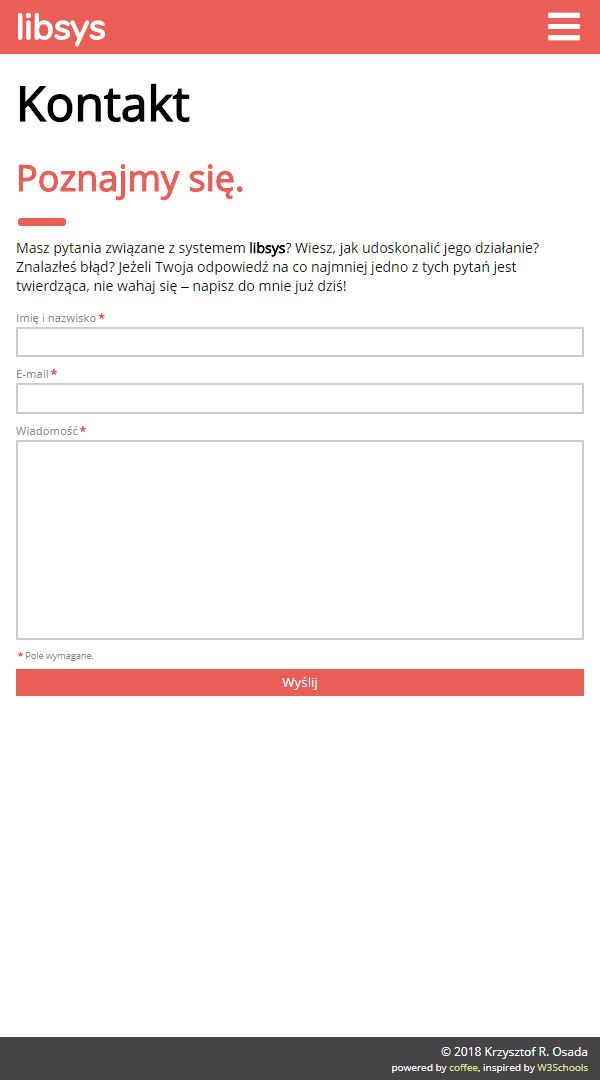
\includegraphics[width=.75\linewidth]{img/libsys_contact.png}
\end{subfigure}
    \caption{\texttt{libsys} -- zmiana hasła / kontakt.}
    \label{fig:libsys_contact}
\end{figure}

Miłym udogodnieniem jest także interaktywna \textbf{mapa} (rys. \ref{fig:libsys_map}), która wskazuje obecne położenie użytkownika i prezentuje lokalizacje wszystkich filii Miejskiej Biblioteki Publicznej we Wrocławiu; każdy oddział jest zaznaczony specjalnym znacznikiem zawierającym informacje nt. danego miejsca.

\begin{figure}[h]
    \centering
    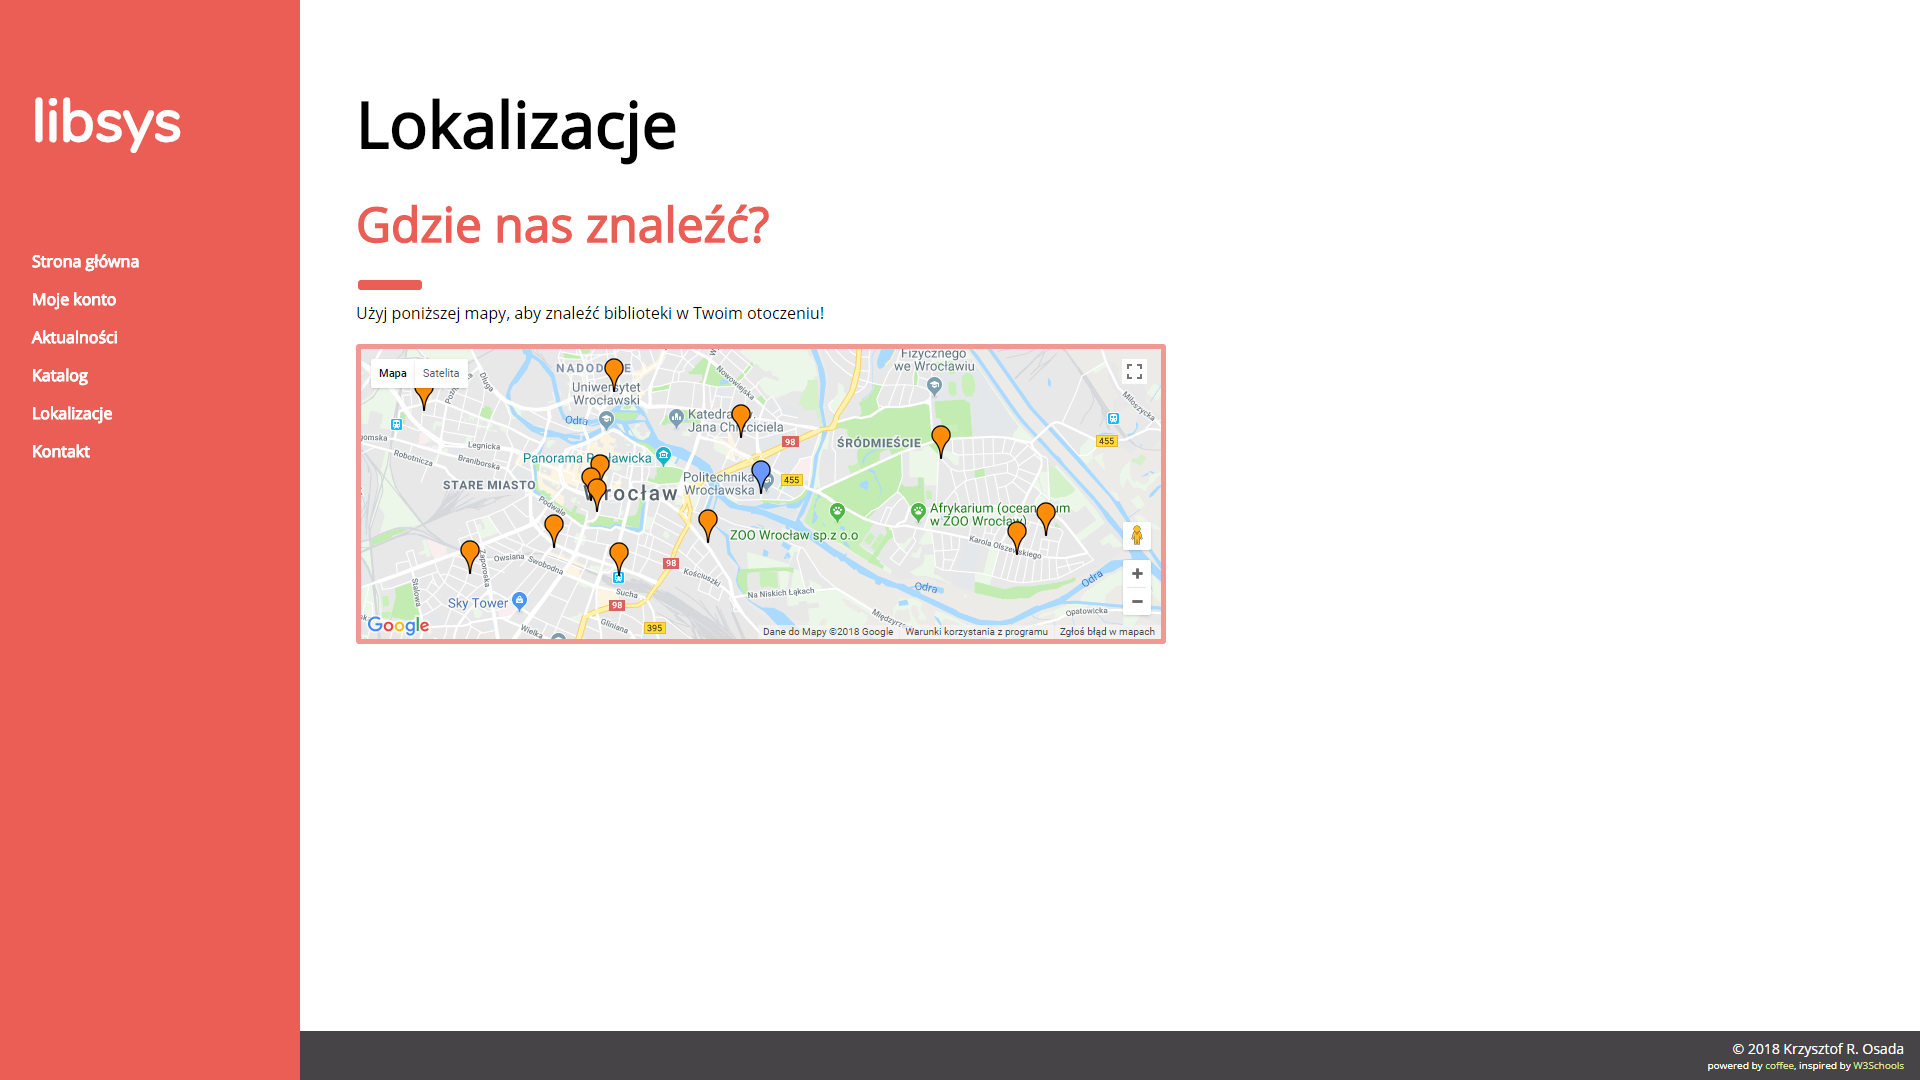
\includegraphics[width=.75\textwidth]{img/libsys_map.png}
    \caption{\texttt{libsys} -- mapa.}
    \label{fig:libsys_map}
\end{figure}

Jedną z najważniejszych części systemu (zgodnie z jego zastosowaniem) jest \textbf{katalog} książek; w podstawowym widoku prezentowane są wszystkie pozycje należące do księgozbioru. Wykaz jest podzielony tak, że w danej chwili wyświetlanych jest co najwyżej 10 pozycji, kolejne zaś -- na następnych stronach. Ważną informacją zarówno dla bibliotekarza, jak i dla czytelnika jest status książki reprezentowany kolorem:

\begin{itemize}
    \item czerwonym     -- trwa wypożyczenie książki (nie została jeszcze zwrócona);
    \item pomarańczowym -- jeden z czytelników dokonał rezerwacji (zamówienia) książki;
    \item zielonym      -- książka jest obecnie dostępna.
\end{itemize}

Użytkownik mający rozszerzone uprawnienia (np. bibliotekarz) może dodawać nowe książki do księgozbioru -- czynność ta wymaga wypełniania formularza z podstawowymi danymi nt. pozycji (imię i nazwisko autora, tytuł, numer ISBN itd.).

\begin{figure}[h]
\centering
\begin{subfigure}{.48\textwidth}
    \centering
    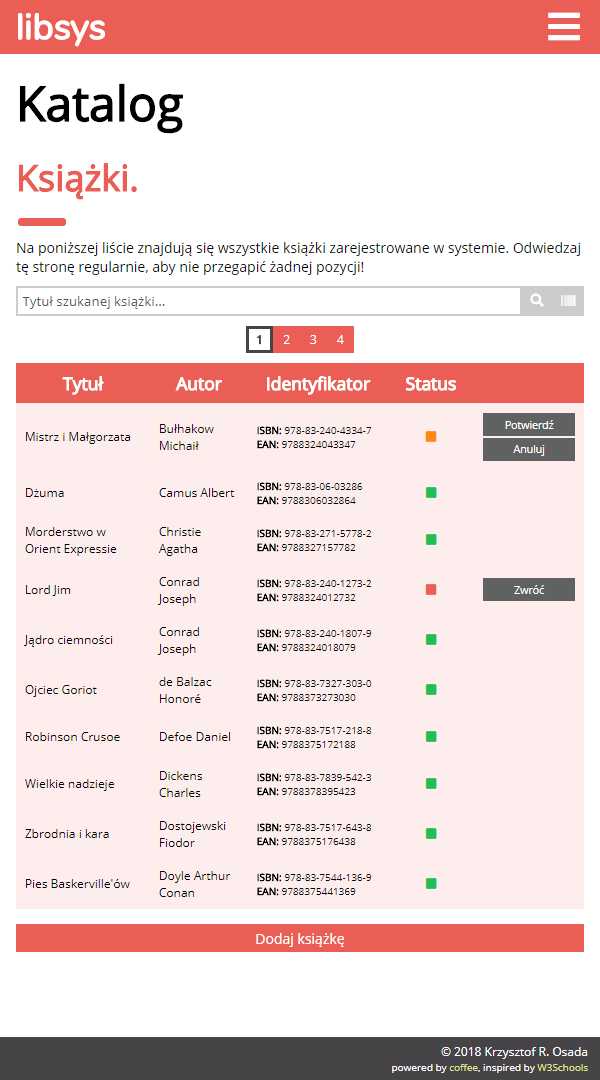
\includegraphics[width=.75\linewidth]{img/libsys_catalog_1.png}
\end{subfigure}\quad
\begin{subfigure}{.48\textwidth}
    \centering
    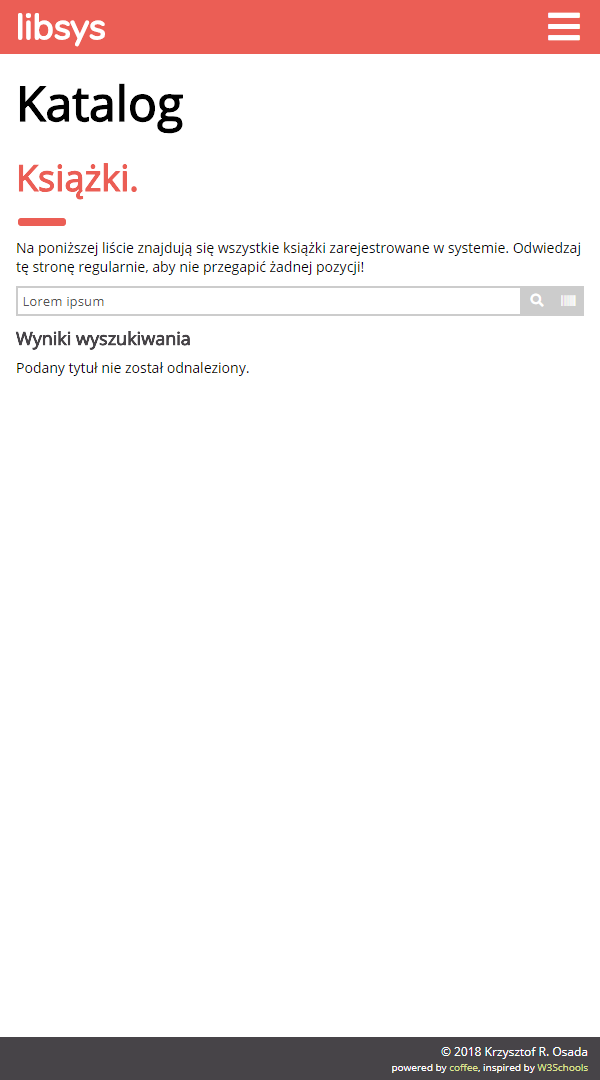
\includegraphics[width=.75\linewidth]{img/libsys_catalog_2.png}
\end{subfigure}
    \caption{\texttt{libsys} -- katalog: lista i wyniki wyszukiwania.}
    \label{fig:libsys_search_results}
\end{figure}

Powyżej listy książek znajduje się \textbf{wyszukiwarka} -- system szuka książki o tytule zgodnym (lub częściowo zgodnym, tzn. zawierającym) z zawartością tego pola i prezentuje ewentualne wyniki w tej samej formie, w jakiej wyświetlany jest księgozbiór (bez podziału na strony). Jeżeli dane zapytanie nie zwróci żadnych rezultatów, to pojawi się stosowny komunikat (rys. \ref{fig:libsys_search_results}).

Praktyczną opcją -- szczególnie z punktu widzenia użytkowników smartfonów -- jest wyszukiwanie książek na bazie \textbf{kodów kreskowych}. Jeśli wybrany przez czytelnika plik zawiera kod kreskowy, to zostaje on sczytany i~porównany z zasobami przechowywanymi w bazie danych; w przypadku niepowodzenia użytkownik zostaje poproszony o załadowanie kolejnej fotografii (przygotowanej wcześniej bądź wykonanej przed chwilą).

\begin{figure}[h]
\centering
\begin{subfigure}{.48\textwidth}
    \centering
    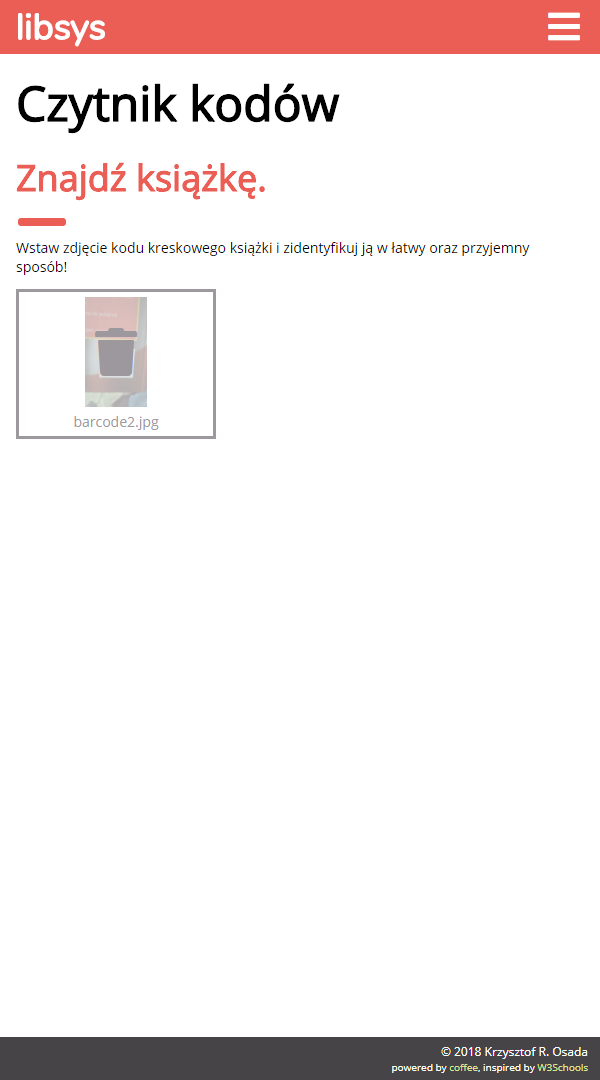
\includegraphics[width=.75\linewidth]{img/libsys_catalog_3.png}
\end{subfigure}\quad
\begin{subfigure}{.48\textwidth}
    \centering
    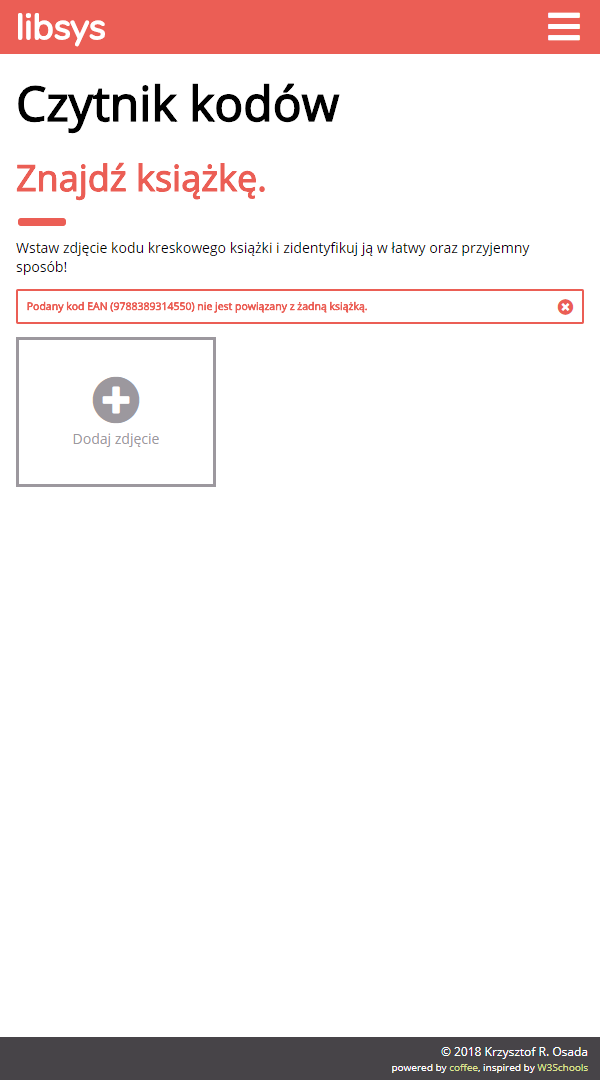
\includegraphics[width=.75\linewidth]{img/libsys_catalog_4.png}
\end{subfigure}
    \caption{\texttt{libsys} -- katalog: wyszukiwanie przy użyciu kodu kreskowego.}
\end{figure}

Może się też zdarzyć, że skrypt nie znajdzie kodu kreskowego na zdjęciu -- w takim wypadku wskazane jest dodanie nowej fotografii albo wpisanie tytułu w wyszukiwarce. Jeśli jednak identyfikacja zasobu bibliotecznego zakończy się pomyślnie, to nastąpi przekierowanie na podsronę podsumowującą informacje o danej książce, w tym jej status -- na podstawie tej zmiennej oraz roli użytkownika (bibliotekarz czy nie-bibliotekarz) system decyduje, które operacje (wypożyczenie, rezerwacja itp.) są dozwolone, a które nie.

\newpage
\section{Podsumowanie}
Niniejszy dokument przybliża główne idee systemu, proponowane funkcjonalności oraz projekt interfejsu graficznego. Istnieje wiele dalszych kierunków rozwoju \texttt{libsys}:

\begin{itemize}
    \item wzmocnienie zabezpieczeń systemu;
    \item udoskonalenie głównych komponentów (bibliotecznego, użytkownika);
    \item rozwinięcie systemu o dalsze, dodatkowe funkcjonalności;
    \item zebranie opinii na temat wstępnej wersj isystemu.
\end{itemize}

\end{document}